\documentclass[11pt,english,german]{report}

% Package import, Document Settings
\usepackage[a4paper,inner=3.5cm,outer=2.5cm]{geometry}
\usepackage[english,ngerman]{babel}
\usepackage[utf8]{inputenc}

% Packages
\usepackage{latexsym}
\usepackage[T1]{fontenc}
\usepackage{graphicx}
\usepackage{hyperref}
\usepackage{tabularx}
\usepackage{etoolbox}
\usepackage{fancyhdr}
\usepackage{amsthm}
\usepackage{mathtools}
\usepackage[xindy]{glossaries}
\usepackage{hyperref}
\usepackage{lastpage}

% clear default
\fancyhead{}
\fancyfoot{}

\pagestyle{fancy}
\fancyhf{}
\renewcommand{\headrulewidth}{0pt} % optional
\fancyfoot[L]{Chapter: \nouppercase{\leftmark}}
\fancyfoot[R]{\thepage/\pageref{LastPage}}

% Redefine the plain page style, Chpater page
\fancypagestyle{plain}{%
  \fancyhf{}
  \renewcommand{\headrulewidth}{0pt} % optional
  \fancyfoot[R]{\thepage/\pageref{LastPage}}
}

\renewcommand{\chaptermark}[1]{\markboth{\MakeUppercase{#1}}{}}

% Glossar
\newglossaryentry{ATAS}
{
    name=ATAS,
    description={Aplinist Tracker \& Alerting System}
}

\theoremstyle{definition}
\newtheorem{exmp}{Beispiel}[subsection]


\makeglossaries

\setcounter{secnumdepth}{2}
\setcounter{tocdepth}{1}

\begin{document}
\pagestyle{empty} %Keine Kopf-/Fusszeilen auf den ersten Seiten.
\begin{titlepage}
\begin{center}

% Oberer Teil der Titelseite:

\includegraphics[width=0.08\textwidth]{img/bfh_logo.png}\\[1cm]    
\textsc{\LARGE Bern University of Applied Sciences}\\[1.5cm]
\textsc{\Large Bachelor Thesis}\\[0.2cm]
\textsc{\Large Informatik}\\[0.5cm]

% Title
\newcommand{\HRule}{\rule{\linewidth}{0.3mm}}
\HRule \\[0.4cm]
{\huge Alpinist Tracker \& Alerting System}\\[0.3cm]
{\huge \bfseries  ATAS}
\HRule \\[2cm]


\includegraphics[width=0.2\textwidth]{img/atas_logo.png}\\[3cm]    

% Author und Lehrer
\begin{minipage}{0.32\textwidth}
\begin{flushleft} \large
\emph{Autor:}\\
Martin \textsc{Schmidli}\\
\end{flushleft}
\end{minipage}
\hfill
\begin{minipage}{0.32\textwidth}
\begin{flushleft} \large
\emph{Dozent:} \\
Mohamed \textsc{Mokdad}
\end{flushleft}
\end{minipage}
\hfill
\begin{minipage}{0.32\textwidth}
\begin{flushleft} \large
\emph{Experte:}\\
Daniel \textsc{Voisard}\\
\end{flushleft}
\end{minipage}

\vspace{20mm}

% Unterer Teil der Seite
Bern, {\large \today}
\end{center}
\end{titlepage}
\pagestyle{fancy}


\tableofcontents


\chapter{Einleitung}
Stellen Sie sich ein kleines mobiles Gerät vor, nachfolgend Tracker genannt, welches Skifahrern, Wanderer usw. abgegeben werden kann. Das Gerät sendet die Position der Person an einen Empfänger, nachfolgend Gateway genannt. Der Gateway wird bei der Talstation oder im nächsten Bergdorf montiert. Der Gateway sendet die empfangenen Daten der Tracker an eine zentrale Stelle irgendwo im Internet. Die Administratoren des Systems, beispielsweise die Rega, können schlussendlich über eine Webseite die aktuelle Position der Personen in den Bergen mitverfolgen und überwachen.

\section{Aufgabenstellung}
Ziel der Bachelorarbeit soll es sein, dass während dem Projekt2 aufgebaute System intensiv zu testen und zu verbessern. Die Arbeit umfasst zwei Hauptaufgaben. Zum einen Teil soll der Tracker in realer Umgebung getestet werden bspw. während einer Wanderung. Die Messdaten werden erfasst und analyisert. Zum anderen soll der Tracker Prototyp verbessert werden; Reichweite, Aufbau, Verlässlichkeit usw. Die dazu erforderlichen Massnahmen werden während der Bachelorarbeit spezifiziert und umgesetzt. Am Ende der Arbeit soll eine klare Aussage gemacht werden können ob das erdachte System praxistauglich ist.


\section{Rahmenbedingungen}
Die Rahmenbedingungen dieses Projektes wurden gemeinsam mit dem Betreuer definiert
\begin{itemize}
\item Die Bachelorarbeit baut auf der Arbeits des Projekt 2 auf. Die erstellete Hard und Software wird weiterverwendet.
\item The Things Network dient als Plattform für die Kommunikation unter den Komponenten.
\item Als Programmiersprache soll C/C++ verwendet werden
\item Auf den Einsatz eines Betriebsystememes auf dem Tracker Node soll verzichtet werden
\end{itemize}

\chapter{Systembeschreibung}
Um die nachfolgenden Kapitel zu verstehen, ist es sehr wichtig, sich mit der im Projekt 2 erstellten Systemarchitektur und die Terminologie vertraut zu machen. Die Architektur wurde im vergleich zum Projekt 2 um einige Komponenten ergänzt.

\section{Grobe Systemarchitektur}
Dieser Abschnitt bietet Ihnen einen groben Überblick über die Benutzer, die Komponeneten und deren Beziehung innerhalb des ATAS Systems. Alle Einheiten werden auf den nachfolgenden Seite detailiert beschrieben.

\newpage
\subsection{Aufbau}
\subsection{Diagram}

\subsection{Benutzer}
Die nachfolgenden Gruppen wurden als Benutzer des Systems identifiziert.
\subsubsection{Aplinist}
Alpinist wird als Generalisierung für Personen, welche sich in den Bergen aufhalten verwendet. Dazu gehören bspw. Wanderer, Skifahrer, Bergbauer usw.
\subsubsection{Überwacher}
Rettungsdienste wie bspw. die Rega oder die AirGlacier. Spitäler oder die lokalen Tourismusbehörden.

\subsection{Komponenten}
Das ATAS System besteht aus den nachfolgenden Komponenten. Komponenten sind als Hardware und Software zu verstehen.
\subsubsection{Tracker}
Stellen Sie sich ein kleines mobiles Gerät vor, nachfolgend genannt Tracker. Der Alpinist trägt den Tracker bei sich bspw. in einem Rucksack.\\ \bigskip
Der Tracker verfügt über ein Display, Taste und ein Lautsprecher. Mit dem druck auf den Knopf können die Überwacher über eine Notsituation aufmerksam gemacht werden. Bspw. Wenn der Alpinist einen Unfall hatte und nun bewegungsunfähig ist.\\ \bigskip
Über den Lautsprecher kann der Aplinist über eine Gefahrenquelle mit einem akustischen Signal aufmerksam gemacht werden. Bspw. Wenn sich der Aplinist in einem Bereich am Berg mit erhöhter Gefahr für Lawinen aufhält. \\ \bigskip
Über ein Display können mehr Informationen zum Tracker und den Gefahrenzonen agezeigt werden. \\ \bigskip
Der Tracker verfügt über ein GPS Modul. Mit dem GPS Modul kann die Position des Tracker auf der Erde ermittelt werden.

\subsubsection{Gateway}

\subsubsection{Broker}

\subsubsection{Wepapplikation}

\subsubsection{Business Logik}

\chapter{Vorgehen}
Das Bachelorarbeit wird in 2 Hauptaufgaben aufgeteilt.\textbf{ Testing} und das erstellen eines zweiten Prototyps nachfolgend genannt \textbf{Prototyp 2}.
\section{Testing}
Ein Teil des Systemaufbaus aus dem vorgängigen Projekt soll getestet werden.\\[0.3cm]
In diesem Kapitel wird genau beschrieben, wie beim Testing des Systems vorgegangen wird.
Das Testing erfolgt in den in der nächsten Abbildung beschriebenenen Schritten.
\begin{figure}[h]
	\centering
	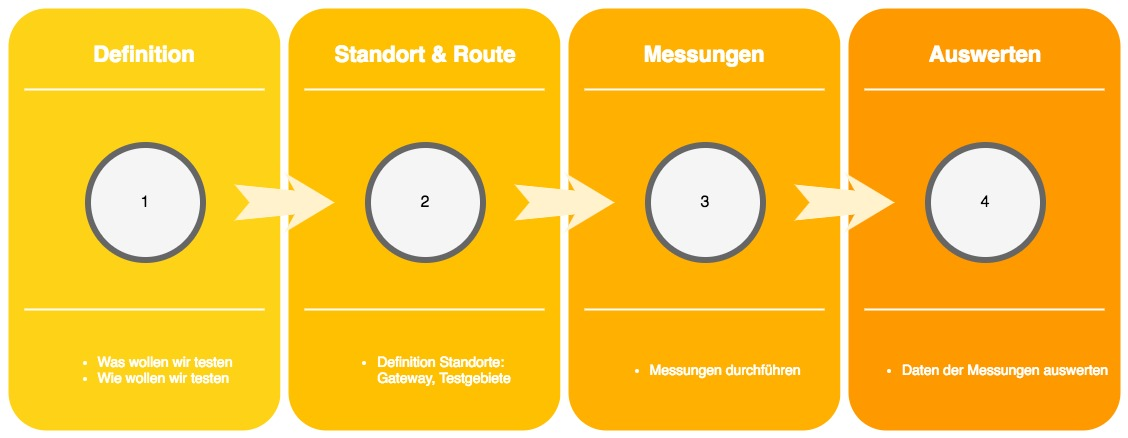
\includegraphics[width=\textwidth]{img/projectFlow_testing.jpg}
	\caption[Flowchart Testing]
	{Ablauf Testing}
\end{figure}
\\ 
Wie genau das Testing definiert wurde, wird in den nächsten Abschnitten beschrieben.

\newpage
\subsection{Definition}
Es muss definiert werden
\begin{itemize}
	\item welche Komponenten geprüft werden bspw. Atas-Node. Atas-Service
	\item welcher Teil der Komponente geprüft werden soll bspw. Kommunikation, Software ..
	\item welche Aspekte betrachtet werden bspw. Sicherheit, Zuverlässigkeit usw.
	\item mit welchen Mitteln resp. Messinstrumenten gemessen wird
\end{itemize}
Während der Arbeit soll die Kommunikation zwischen Atas-Node und Atas-Gateway getestet werden. Der Fokus liegt auf der Zuverlässigkeit der Übertragung. Mich interessiert, wie sicher es ist, dass eine Meldung ihr Ziel erreicht.\\[0.3cm]
Ausgehend von den Definitionen müssen verschiedene Testszenarios erstellt werden. 

\subsection{Standort}
Ausgehend von den vorangegangen Definitionen muss folgendes definiert werden.
\begin{itemize}
	\item Es muss ein Ort gefunden werden, wo der Gateway platziert werden soll. Der Standort kann frei gewählt werden. Einzige Vorraussetzungen ist ein Zugang zum Internet.
	\item Für die Tests sollen mind. 2 Wege / Pfade definiert werden. Da die Zielgruppe des Trackers die Alpinisten sind, sollten die Pfade  Auf dem Pfad selbst werden 5 Orte definiert wo die Verbindungstests durcheführt werden.
\end{itemize}
	
\subsection{Messungen}
Die vorgängig definierten Routen werden abgelaufen und die Messungen werden an den definierten Standorten durchgeführt.

\subsection{Auswertung}
Die erhobenen Daten werden analysiert.

\newpage
\section{Prototyp 2}
\begin{figure}[h]
	\centering
	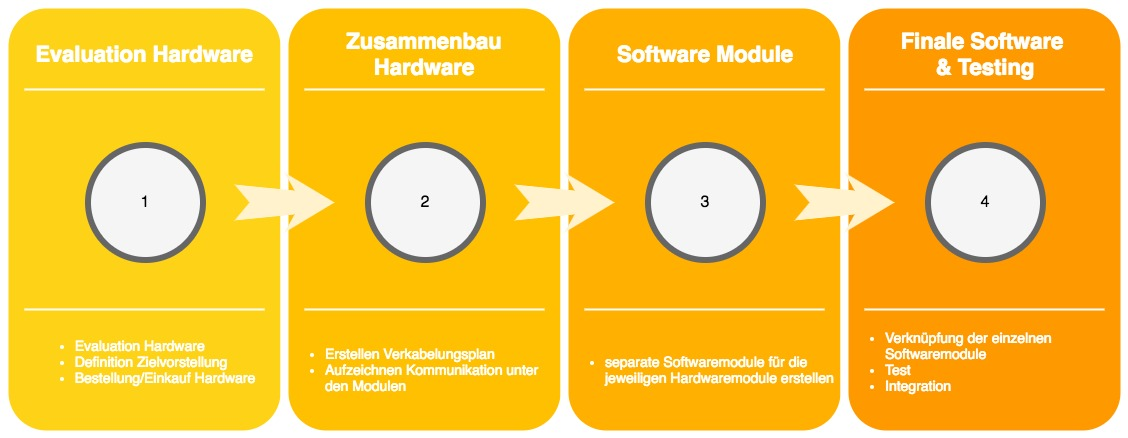
\includegraphics[width=\textwidth]{img/projectFlow_hardware.jpg}
	\caption[Flowchart Prototyp 2]
	{Ablauf für den Aufbau des zweiten Prototyps}
\end{figure}




- Portieren der Software auf ES32
- 
- TTN als Platform
- SPI Schnittstelle analyse, was schickt die Lorwan library
- Bitrate + laufzeit Analyse
- Minimierung 


\chapter{Testing}
\section{Aufbau Gateway}
Code:
apt-get update
apt-get upgrade

%sudo dpkg-reconfigure locales // de_CH
sudo dpkg-reconfigure tzdata // Europe/Zurich

sudo raspi-config // Enable SPI

git clone https://github.com/ttn-zh/ic880a-gateway.git ~/ic880a-gateway
cd ~/ic880a-gateway

change EUI Source to Wireless
%GATEWAY_EUI_NIC="wlan0"

sudo ./install.sh spi


\chapter{Prototyp}
\section{Entwicklungsumgebung}
Installation gemäss Anleitung auf dieser Webseite:\\
\url{https://dl.espressif.com/doc/esp-idf/latest/get-started/index.html}\\
Treiber für MacOs:\\
\url{https://www.silabs.com/products/development-tools/software/usb-to-uart-bridge-vcp-drivers}
\section{Hardware}
Für den Aufbau des Prototypen wurde die nachfolgende Hardware verwendet

\begin{table}[htbp]
    \centering
	\begin{tabularx}{\textwidth}{lll}
		Name & Gerätetyp & Bild \\ \hline
		Espressfif ESP32 & Entwicklungbaord & to be created\\ \hline
	\end{tabularx}
\end{table}

\chapter*{Selbständigkeitserklärung}
\label{chap:selbstaendigkeitserklaerung}

\vspace*{10mm} 

Ich bestätige, dass ich die vorliegende Arbeit selbstständig und ohne Benutzung anderer als der im Literaturverzeichnis angegebenen Quellen und Hilfsmittel angefertigt habe. Sämtliche Textstellen, die nicht von mir stammen, sind als Zitate gekennzeichnet und mit dem genauen Hinweis auf ihre Herkunft versehen. 

\vspace{15mm}

\begin{tabbing}
xxxxxxxxxxxxxxxxxxxxxxxxx\=xxxxxxxxxxxxxxxxxxxxxxxxxxxxxx\=xxxxxxxxxxxxxxxxxxxxxxxxxxxxxx\kill
Ort, Datum:\> Bern, 15.01.2018 \\ \\
Namen Vornamen:\> Martin Schmidli  \\ \\ \\ \\ 
Unterschriften:\> ...................................... \\
\end{tabbing}

\chapter*{Anhang}
\section{Software}
Es wird kein Code direkt an dieses Dokument angehängt. Jegliche Commits vor dem 16.09.2017 gehören zur Projekt 2 Arbeit. Commits nach diesem Datum wurden im Zuge der Bachelor Thesis erstellt. Der Code der ATAS Softwarekomponenten wurde auf die Plattform github hochgeladen. Folgend Sie den Links um den Sourcecode einzusehen.
\subsection{Atas-Webapp}
\url{https://github.com/schmm2/atas-webapp}
\subsection{Atas-Node}
\url{https://github.com/schmm2/atas-node}
\subsection{Atas-Service}
\url{https://github.com/schmm2/atas-service}


\printglossaries

\end{document}